\documentclass[border=0pt]{standalone}
% Shared visual language for CAML diagrams (pdflatex + Fira Sans/Mono).
% Native SVG output: build with latex (DVI) + dvisvgm, see build.sh. The
% PDF route (pdflatex + dvisvgm --pdf) turns every transparency into solid
% black/white blocks.
\def\pgfsysdriver{pgfsys-dvisvgm.def}
\usepackage[T1]{fontenc}
\usepackage[sfdefault]{FiraSans}
\usepackage[scale=0.92]{FiraMono}
\usepackage{amssymb}
\usepackage{tikz}
\usetikzlibrary{arrows.meta, positioning, shadows, fit, backgrounds, calc}

% --- palette ------------------------------------------------------------
\definecolor{ink}{HTML}{16202C}
\definecolor{muted}{HTML}{5B6B7F}
\definecolor{edge}{HTML}{47576B}
\definecolor{card}{HTML}{F7F9FC}
\definecolor{page}{HTML}{FFFFFF}

\definecolor{indigo}{HTML}{4B54C6}   \definecolor{indigobg}{HTML}{EDEEFC}
\definecolor{amber}{HTML}{C9740A}    \definecolor{amberbg}{HTML}{FCF0DE}
\definecolor{green}{HTML}{0E9E6B}    \definecolor{greenbg}{HTML}{E4F6EE}
\definecolor{purple}{HTML}{7A3CE0}   \definecolor{purplebg}{HTML}{F1E9FD}
\definecolor{rose}{HTML}{D23F72}     \definecolor{rosebg}{HTML}{FBE7EE}
\definecolor{slate}{HTML}{47576B}    \definecolor{slatebg}{HTML}{EDF1F6}

% --- node + arrow styles ------------------------------------------------
% A flat offset drop shadow: shadows.blur's faded shadows render as solid
% black boxes under the dvisvgm driver.
\tikzset{soft shadow/.style={drop shadow={shadow xshift=0pt, shadow yshift=-1.8pt,
                                          opacity=0.12, fill=ink}}}
\tikzset{
  base/.style={
    rounded corners=5pt, draw, line width=1pt, inner sep=8pt,
    font=\small, text=ink, align=center,
    soft shadow},
  card/.style   ={base, fill=card,     draw=muted!70},
  indigo/.style ={base, fill=indigobg, draw=indigo, text=ink},
  amber/.style  ={base, fill=amberbg,  draw=amber,  text=ink},
  green/.style  ={base, fill=greenbg,  draw=green,  text=ink},
  purple/.style ={base, fill=purplebg, draw=purple, text=ink},
  rose/.style   ={base, fill=rosebg,   draw=rose,   text=ink},
  slate/.style  ={base, fill=slatebg,  draw=slate,  text=ink},
  sub/.style={font=\scriptsize, text=muted},
  arrow/.style={-{Stealth[length=2.8mm,width=2.4mm]}, line width=1.1pt, draw=edge},
  arrowd/.style={-{Stealth[length=2.8mm,width=2.4mm]}, line width=1.1pt, draw=edge, dashed},
  alabel/.style={font=\scriptsize, text=muted, align=center, fill=page, inner sep=2pt},
  grouplbl/.style={font=\bfseries\footnotesize, text=ink},
}

% inline text helpers for two-tier node labels
\newcommand{\Hd}[1]{{\bfseries #1}}
\newcommand{\Sb}[1]{{\normalfont\scriptsize\textcolor{muted}{#1}}}
\newcommand{\Sbc}[2]{{\normalfont\scriptsize\textcolor{#1}{#2}}}

% White rounded card behind every diagram. The SVGs used to be transparent
% with dark ink, so labels drawn straight on the page vanished on GitHub's
% dark theme. It is drawn on its own lowest layer: the backgrounds
% library's `show background rectangle` would cover anything a diagram puts
% `on background layer` (pipeline.tex's sandbox box). banner.tex opts out
% with \camlcardfalse since it is its own dark card.
\newif\ifcamlcard \camlcardtrue
\pgfdeclarelayer{card}
\pgfsetlayers{card,background,main}
\tikzset{every picture/.append style={execute at end picture={%
  \ifcamlcard
    \begin{pgfonlayer}{card}
      \path[fill=page, draw=muted!22, line width=0.6pt, rounded corners=12pt]
        ([shift={(-12pt,-12pt)}]current bounding box.south west) rectangle
        ([shift={(12pt,12pt)}]current bounding box.north east);
    \end{pgfonlayer}
  \fi}}}

\camlcardfalse % the banner is its own dark card
\definecolor{night}{HTML}{0D1224}
\definecolor{night2}{HTML}{151B33}
\definecolor{term}{HTML}{090D1A}
\definecolor{termedge}{HTML}{2A3352}
\definecolor{lilac}{HTML}{A5B4FC}
\definecolor{haze}{HTML}{CBD5E1}
\definecolor{dim}{HTML}{8391A7}
\definecolor{mint}{HTML}{34D399}
\begin{document}
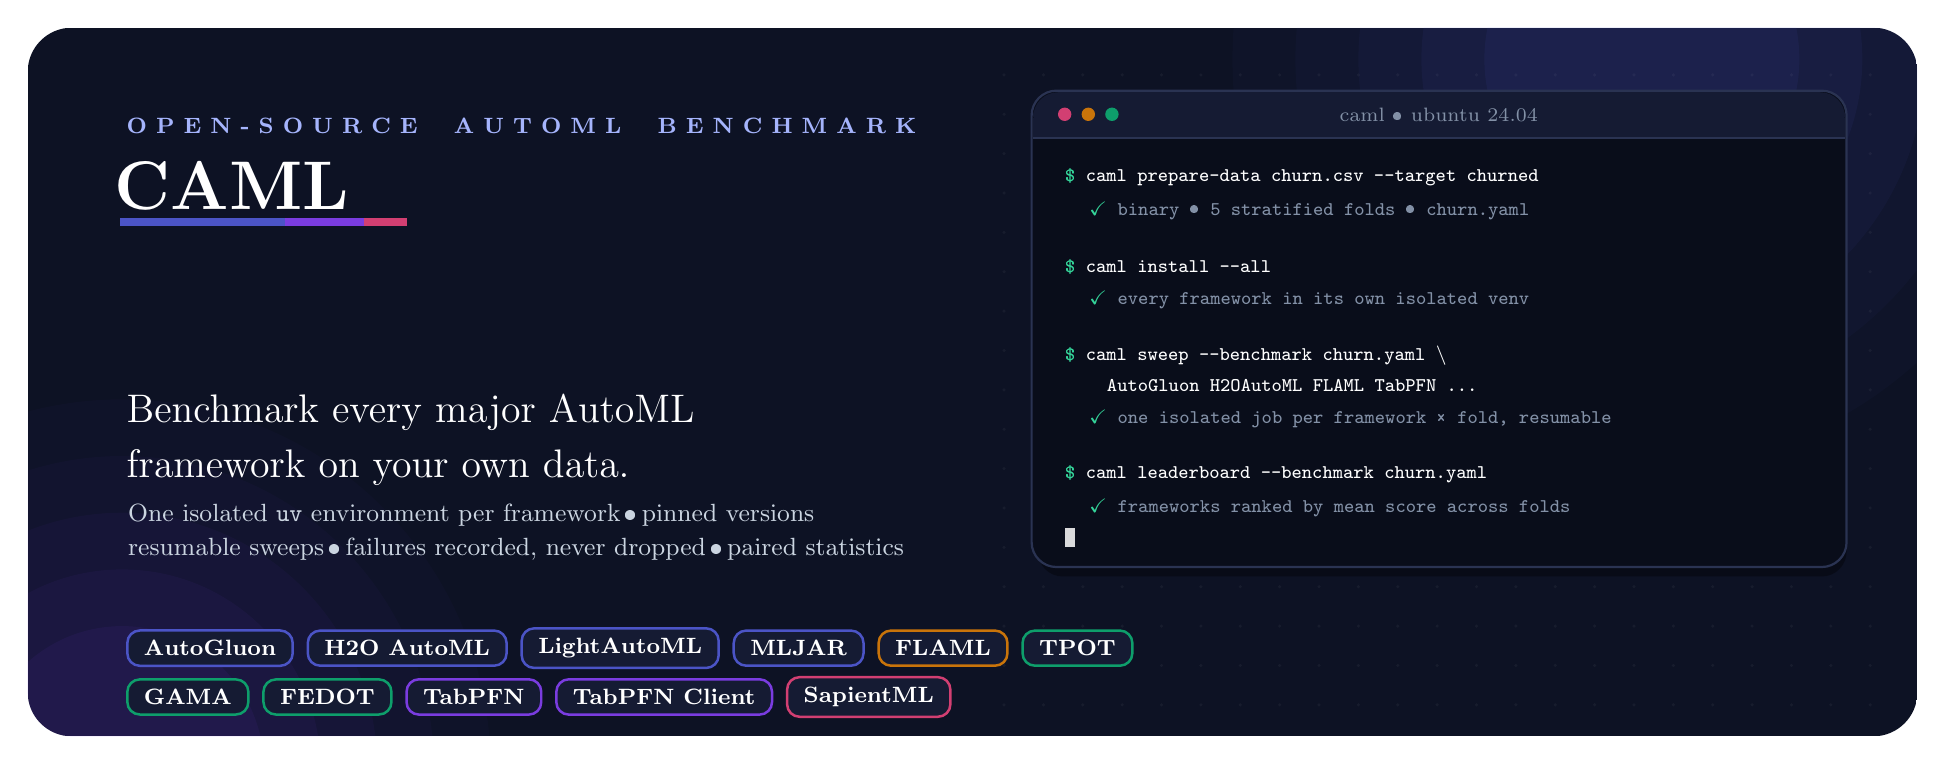
\begin{tikzpicture}[x=1cm, y=1cm,
  fwchip/.style={rounded corners=4.5pt, line width=0.9pt, fill=night2, inner xsep=6pt,
                 inner ysep=3.6pt, font=\fontsize{7.6}{9}\selectfont\bfseries, text=white},
  prompt/.style={anchor=west, font=\ttfamily\fontsize{7.4}{9}\selectfont, text=white, inner sep=0pt},
  okline/.style={anchor=west, font=\ttfamily\fontsize{7.0}{9}\selectfont, text=dim, inner sep=0pt},
]
  % ---- canvas ----------------------------------------------------------
  \clip[rounded corners=16pt] (0,0) rectangle (24,9);
  \fill[night] (0,0) rectangle (24,9);
  % soft glows: stacked translucent discs fake a blur
  \foreach \r/\o in {5.2/0.035, 4.4/0.045, 3.6/0.06, 2.8/0.075, 2.0/0.09}{
    \fill[fill=indigo, opacity=\o] (20.5,8.6) circle (\r);
    \fill[fill=purple, opacity=\o*0.8] (1.2,-0.4) circle (\r*0.9);
  }
  % faint dot grid on the right half
  \foreach \x in {12.4,12.9,...,23.6}{\foreach \y in {0.4,0.9,...,8.6}{
    \fill[white, opacity=0.045] (\x,\y) circle (0.022);}}

  % ---- headline block -------------------------------------------------------
  \node[anchor=north west, inner sep=0pt, text=lilac, font=\fontsize{8.2}{10}\selectfont\bfseries]
    at (1.25,7.85) {O P E N - S O U R C E \quad A U T O M L \quad B E N C H M A R K};
  \node[anchor=north west, inner sep=0pt, text=white, font=\fontsize{66}{66}\selectfont\bfseries]
    (word) at (1.1,7.3) {CAML};
  \fill[fill=indigo] ([xshift=2pt, yshift=-6pt]word.south west) rectangle ++(2.1,0.11);
  \fill[fill=purple] ([xshift=2pt, yshift=-6pt]word.south west) ++(2.1,0) rectangle ++(1.0,0.11);
  \fill[fill=rose]   ([xshift=2pt, yshift=-6pt]word.south west) ++(3.1,0) rectangle ++(0.55,0.11);
  \node[anchor=north west, inner sep=0pt, text=white, align=left,
        font=\fontsize{15.5}{20}\selectfont]
    at (1.25,4.35) {Benchmark every major AutoML\\framework on your own data.};
  \node[anchor=north west, inner sep=0pt, text=haze, align=left,
        font=\fontsize{8.8}{12}\selectfont]
    at (1.27,2.95) {One isolated \texttt{uv} environment per framework\,\textbullet\,pinned versions\\
                    resumable sweeps\,\textbullet\,failures recorded, never dropped\,\textbullet\,paired statistics};

  % ---- terminal card --------------------------------------------------------
  \begin{scope}[shift={(12.75,2.15)}]
    \fill[black, opacity=0.35, rounded corners=9pt] (0.08,-0.12) rectangle (10.35,5.98);
    \fill[term, draw=termedge, line width=0.8pt, rounded corners=9pt] (0,0) rectangle (10.35,6.05);
    \fill[night2, rounded corners=9pt] (0.02,5.45) rectangle (10.33,6.03);
    \fill[night2] (0.02,5.45) rectangle (10.33,5.7);
    \draw[termedge, line width=0.6pt] (0.02,5.45) -- (10.33,5.45);
    \fill[fill=rose]  (0.42,5.75) circle (0.085);
    \fill[fill=amber] (0.72,5.75) circle (0.085);
    \fill[fill=green] (1.02,5.75) circle (0.085);
    \node[font=\fontsize{6.8}{8}\selectfont, text=dim] at (5.17,5.75) {caml \textbullet\ ubuntu 24.04};

    \node[prompt] at (0.42,4.95) {\textcolor{mint}{\$} caml prepare-data churn.csv -{}-target churned};
    \node[okline] at (0.72,4.52) {\textcolor{mint}{$\checkmark$} binary \textbullet\ 5 stratified folds \textbullet\ churn.yaml};
    \node[prompt] at (0.42,3.82) {\textcolor{mint}{\$} caml install -{}-all};
    \node[okline] at (0.72,3.39) {\textcolor{mint}{$\checkmark$} every framework in its own isolated venv};
    \node[prompt] at (0.42,2.69) {\textcolor{mint}{\$} caml sweep -{}-benchmark churn.yaml \textbackslash};
    \node[prompt] at (0.95,2.31) {AutoGluon H2OAutoML FLAML TabPFN ...};
    \node[okline] at (0.72,1.88) {\textcolor{mint}{$\checkmark$} one isolated job per framework \texttimes\ fold, resumable};
    \node[prompt] at (0.42,1.18) {\textcolor{mint}{\$} caml leaderboard -{}-benchmark churn.yaml};
    \node[okline] at (0.72,0.75) {\textcolor{mint}{$\checkmark$} frameworks ranked by mean score across folds};
    \fill[white, opacity=0.85] (0.42,0.25) rectangle ++(0.13,0.24);
  \end{scope}

  % ---- framework chips ------------------------------------------------------
  \begin{scope}[node distance=0.16cm]
    \node[fwchip, draw=indigo, anchor=west] (f1) at (1.25,1.12) {AutoGluon};
    \node[fwchip, draw=indigo, right=of f1] (f2) {H2O AutoML};
    \node[fwchip, draw=indigo, right=of f2] (f3) {LightAutoML};
    \node[fwchip, draw=indigo, right=of f3] (f4) {MLJAR};
    \node[fwchip, draw=amber, right=of f4] (f5) {FLAML};
    \node[fwchip, draw=green, right=of f5] (f6) {TPOT};
  \end{scope}
  \begin{scope}[node distance=0.16cm]
    \node[fwchip, draw=green, anchor=west] (g1) at (1.25,0.5) {GAMA};
    \node[fwchip, draw=green, right=of g1] (g2) {FEDOT};
    \node[fwchip, draw=purple, right=of g2] (g3) {TabPFN};
    \node[fwchip, draw=purple, right=of g3] (g4) {TabPFN Client};
    \node[fwchip, draw=rose, right=of g4] (g5) {SapientML};
  \end{scope}
\end{tikzpicture}
\end{document}
